% Ìmọ̀lára — NLP Summative Project report (ACL style). Compile with XeLaTeX (e.g. `tectonic main.tex`) — see report/README.md.
\documentclass[11pt]{article}
\usepackage[final]{acl}
\usepackage{fontspec}
\setmainfont{texgyretermes}[Extension=.otf, UprightFont=*-regular, BoldFont=*-bold, ItalicFont=*-italic, BoldItalicFont=*-bolditalic]
\usepackage{newunicodechar}
\newunicodechar{ǹ}{\`{n}}
\usepackage{booktabs}
\usepackage{multirow}
\usepackage{graphicx}
\usepackage{xurl}
\usepackage{amsmath}
\usepackage{xcolor}
\usepackage{enumitem}
\setlist{nosep, leftmargin=*}
\graphicspath{{figures/}}  % copies of results/figures/*.png (regenerate with python -m src.figures / src.eda)
\newcommand{\pmstd}[1]{\,{\scriptsize$\pm$#1}}

\title{Ìmọ̀lára: Diacritic-Robust Sentiment Classification for Yorùbá Tweets\\with Classical, Recurrent and Africa-Centric Transformer Models}

\author{Hassan Adelani Luqman \\
  NLP Summative Project — Option 3: Text Classification for an African Language}

\begin{document}
\maketitle

\begin{abstract}
We study three-class sentiment classification (negative, neutral, positive) of Yorùbá tweets, a language spoken by tens of millions of people but poorly served by NLP. Using the AfriSenti-SemEval~2023 Yorùbá data (8,522 / 2,090 / 4,515 tweets), we compare a TF-IDF baseline, BiLSTM/BiGRU models with attention over static embeddings, and six fine-tuned Transformers (mBERT, XLM-R, AfriBERTa, AfroXLMR base/large, and LoRA). Two data problems shape the study: the released test split is pre-normalised while train and dev are raw, and 13\% of dev tweets duplicate training tweets; we reconstruct the normalisation and select models on de-duplicated (``clean'') dev data. Africa-centric pre-training helps (+3.7 macro-F1 from XLM-R to AfroXLMR-base) and the 126M-parameter AfriBERTa is the strongest Transformer (clean-test macro-F1 0.732), yet no model significantly beats the tuned TF-IDF baseline (0.737); a learning curve shows the pre-training advantage shrinks from 4.8 to 0.9 points as labelled data grows. All models trained on diacritised text lose 6--13 points when users type without tone marks; training on all three written forms (\emph{mixed3}) removes almost all of this loss at no cost, giving the best test models (TF-IDF 0.745, AfriBERTa 0.741, weighted-F1 77.8 / 77.5 vs.\ 74.1 for the strongest single model reported with the dataset). Error analysis attributes much of the remaining error to negation, idioms, keyword priors and an estimated 10\% label noise. The diacritic-robust models are deployed in a public web application.
\end{abstract}

\paragraph{Project links.}
\textbf{GitHub:} \url{https://github.com/Hassan-Adelani-Luqman/imolara-yoruba-sentiment} \\
\textbf{Live system:} \url{https://imolara-yoruba-sentiment-oafn6nuzsde8db6a9fdahs.streamlit.app/} \\
\textbf{Model:} \url{https://huggingface.co/Hassanadelani1/imolara-afriberta-mixed3} \\
\textbf{Demo video:} \textcolor{red}{[link to be added]}

\section{Introduction}
Sentiment analysis of social-media text supports public-opinion monitoring, customer-feedback triage and social research. For most African languages such tools hardly exist: Yorùbá, spoken by roughly 50 million people in Nigeria, Benin and the diaspora \citep{eberhard-etal-2025-ethnologue}, has a small fraction of the labelled resources of high-resource languages \citep{joshi-etal-2020-state}. The NaijaSenti and AfriSenti projects \citep{muhammad-etal-2022-naijasenti,muhammad-etal-2023-afrisenti} created the first sizeable annotated Yorùbá Twitter corpus and a shared task \citep{muhammad-etal-2023-semeval}, so the task itself is established; what is missing is (i) a systematic, statistically careful comparison of classical, recurrent and Transformer approaches on this data, (ii) an account of how models behave under the way Yorùbá is actually typed, and (iii) a usable tool.

Written Yorùbá marks tone with grave and acute accents and vowel quality with an under-dot (\emph{ẹ, ọ, ṣ}); in electronic text these diacritics are frequently omitted \citep{orife-2018-attentive}, which makes words ambiguous (\emph{èdè} `language' vs.\ \emph{edé} `crayfish', both written \emph{ede}) and changes model behaviour \citep{adelani-etal-2021-effect}. Most AfriSenti Yorùbá tweets are diacritised (77\%, §\ref{sec:data}), but a deployed classifier will meet input from phone keyboards without them.

\paragraph{Objective and research questions.} We build and deploy a three-class Yorùbá tweet sentiment classifier and ask:
\textbf{RQ1} Do Africa-centric pre-trained models outperform general multilingual models and classical baselines?
\textbf{RQ2} How robust are models to tweets written without tone marks or without any diacritics, and can training fix it?
\textbf{RQ3} Does training data from related Nigerian languages (Hausa, Igbo, Pidgin) help?

\paragraph{Contributions.} (1) We identify and correct a train/test format mismatch in the released data and quantify train/dev/test duplication; (2) we compare more than 30 model configurations, with three seeds for every neural model, bootstrap confidence intervals and paired significance tests; (3) we show that diacritic augmentation makes models robust to undiacritised input at no cost; (4) we analyse errors with reproducible evidence (keyword slices, duplicate-label conflicts, confident learning); (5) we deploy the models in a public web application with a validated int8 ONNX model.

\section{Related Work}
\paragraph{African-language sentiment.} NaijaSenti \citep{muhammad-etal-2022-naijasenti} annotated tweets in Hausa, Igbo, Nigerian Pidgin and Yorùbá; AfriSenti \citep{muhammad-etal-2023-afrisenti} extended this to 14 languages and reported single-model baselines, the best for Yorùbá being AfroXLMR-large (74.1 weighted-F1) and AfriBERTa-large (72.9). In the SemEval-2023 shared task \citep{muhammad-etal-2023-semeval}, the best Yorùbá systems reached about 80 weighted-F1, typically with additional language- and task-adaptive pre-training and ensembling \citep{wang-etal-2023-nlnde}. These works establish strong numbers but do not study robustness to diacritic variation, the train/test format difference, or duplicate leakage, and they do not provide an end-user tool.

\paragraph{Pre-trained models for African languages.} General multilingual encoders such as mBERT \citep{devlin-etal-2019-bert} and XLM-R \citep{conneau-etal-2020-unsupervised} cover few African languages; XLM-R's CC-100 pre-training data contains no Yorùbá. AfriBERTa \citep{ogueji-etal-2021-small} is trained from scratch on under 1\,GB of text in 11 African languages; AfroXLMR \citep{alabi-etal-2022-adapting} adapts XLM-R to 17 African languages by multilingual adaptive fine-tuning; SERENGETI \citep{adebara-etal-2023-serengeti} covers 517 African languages. Comparing XLM-R and AfroXLMR, which share architecture and tokenizer, isolates the effect of African pre-training data (RQ1).

\paragraph{Diacritics in Yorùbá NLP.} \citet{orife-2018-attentive} frames missing diacritics as a restoration task; \citet{adelani-etal-2021-effect} show diacritics affect Yorùbá--English translation quality. We instead make classifiers \emph{invariant} to diacritic variation by data augmentation, a simpler alternative to a restoration pipeline.

\paragraph{Models and evaluation.} Our recurrent models follow LSTMs \citep{hochreiter-schmidhuber-1997-lstm}, GRUs \citep{cho-etal-2014-learning} and additive attention \citep{bahdanau-etal-2015-neural} over Word2Vec \citep{mikolov-etal-2013-efficient} or fastText vectors \citep{bojanowski-etal-2017-enriching,grave-etal-2018-learning}. For parameter-efficient fine-tuning we use LoRA \citep{hu-etal-2022-lora}. Fine-tuning large encoders is known to be unstable across seeds \citep{mosbach-etal-2021-stability}, which motivates our multi-seed protocol; significance is assessed with the paired bootstrap \citep{koehn-2004-statistical,efron-tibshirani-1993-bootstrap}, and label noise with confident learning \citep{northcutt-etal-2021-confident}.

\section{Dataset and Data Preparation}\label{sec:data}
\paragraph{Source and size.} We use the Yorùbá portion of AfriSenti-SemEval~2023 \citep{muhammad-etal-2023-afrisenti,afrisenti-github} (CC BY 4.0), whose tweets were annotated by three native speakers each with majority voting; free-marginal agreement for Yorùbá is $\kappa = 0.65$. We download the raw TSVs pinned to a fixed repository commit (the Hugging Face copy relies on a loading script that current libraries no longer execute). Table~\ref{tab:data} gives the official splits. Negative is the minority class (22\%), so macro-F1 is our primary metric.

\begin{table}[t]
\centering\small
\begin{tabular}{lrrrr}
\toprule
Split & Tweets & Negative & Neutral & Positive \\
\midrule
Train & 8,522 & 1,872 & 3,108 & 3,542 \\
Dev   & 2,090 &   443 &   763 &   884 \\
Test  & 4,515 &   981 & 1,616 & 1,918 \\
\bottomrule
\end{tabular}
\caption{AfriSenti Yorùbá splits. \emph{Clean} subsets without duplicates of training tweets: 1,817 dev and 4,129 test tweets. (The dataset paper's counts include the TSV header line.)}
\label{tab:data}
\end{table}

\paragraph{Exploratory analysis.} Tweets are short (median 18 tokens after normalisation; 95th percentile 45). 77\% contain tone marks and 73\% under-dots, and diacritic presence correlates with the label (85\% of neutral vs.\ 71\% of negative tweets carry tone marks), a potential shortcut cue. A heuristic English detector flags about 14\% of tweets as code-switched. Test is lexically further from train than dev: 41\% of test word types are unseen in training (dev: 29\%); ignoring diacritics shrinks the vocabulary by about 30\% and lowers the token OOV rate from 7.8\% to 5.2\%.

\paragraph{A train/test format mismatch.} The released test split is pre-normalised (0\% uppercase, punctuation, hashtags or URLs, 0.5\% emojis) while train and dev are raw tweets (e.g.\ 99\% uppercase, 57\% hashtags; Figure~\ref{fig:surface}). We reconstruct the organisers' normalisation---lower-casing and removing mentions, URLs, \texttt{RT}, hashtags (with their word), apostrophes, digits, punctuation and emojis, keeping letters and combining marks---and validate it on train/test pairs that are the same tweet: it reproduces 76 of 79 test strings exactly (the three misses differ in the underlying tweet). We apply it, after Unicode NFC normalisation, to every split, in training and in the deployed application.

\begin{figure}[t]
\centering
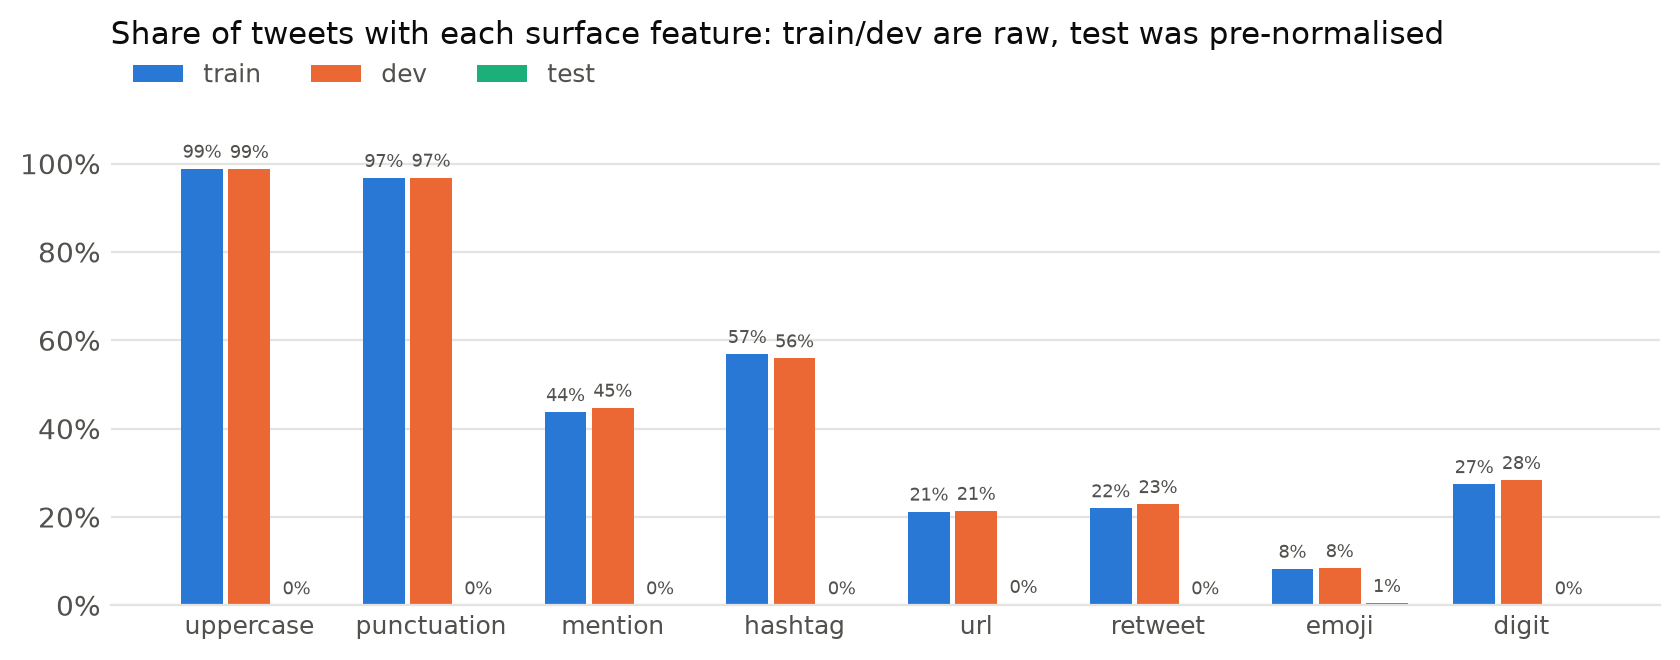
\includegraphics[width=\columnwidth]{eda_surface_features.png}
\caption{Share of tweets with each surface feature: train/dev are raw, the released test split was pre-normalised.}
\label{fig:surface}
\end{figure}

\paragraph{Duplicates and leakage.} Comparing tweets after normalisation and diacritic removal, 13.1\% of dev (273) and 8.5\% of test tweets (386) duplicate a training tweet---retweets, reposted proverbs, or the same tweet with different hashtags. Duplicates inflate dev scores by about 3 points and bias model selection towards memorisation. We keep the official splits for comparability but report every result on the full split and on a \emph{clean} subset without duplicates, and select models on \textbf{clean dev}.

\paragraph{Diacritic forms and auxiliary data.} For RQ2 every tweet can be rendered in three forms: \emph{original}, \emph{no tones} (combining grave, acute and macron removed; under-dots kept) and \emph{no diacritics} (all combining marks removed). For RQ3 we use the AfriSenti Hausa (14,172), Igbo (10,192) and Pidgin (5,121) training sets; Pidgin is only 1.4\% neutral. No synthetic or LLM-generated data is used.

\section{Methodology}
\paragraph{Baselines (E0--E1).} A majority-class predictor, and TF-IDF features (sublinear tf, $\textit{min\_df}=2$) of word 1--2-grams, character 2--5-grams (\texttt{char\_wb}) or their union, with logistic regression or a linear SVM \citep{pedregosa-etal-2011-scikit}. $C$ and class weighting are grid-searched on clean dev. Word tokens are split on whitespace: scikit-learn's default token pattern drops one-letter words such as \emph{o} and breaks words at combining tone marks (\emph{ọ̀rẹ́}~$\rightarrow$~\emph{rẹ}).

\paragraph{Recurrent models (E2).} Tokens are embedded (300-d), passed through a bidirectional LSTM or GRU (hidden size $h=128$ per direction) giving states $H=[\mathbf{h}_1,\dots,\mathbf{h}_T]$, pooled by additive attention \citep{bahdanau-etal-2015-neural},
\begin{gather*}
\alpha_t = \operatorname{softmax}_t\!\left(\mathbf{v}^{\top}\tanh(W\mathbf{h}_t)\right),\\
\mathbf{c}=\textstyle\sum_t \alpha_t\mathbf{h}_t ,
\end{gather*}
and classified by a linear layer over $\mathbf{c}$ (ablation: concatenated final states). Embeddings are random, pre-trained fastText Yorùbá vectors \citep{grave-etal-2018-learning}, or our own skip-gram Word2Vec \citep{mikolov-etal-2013-efficient} trained with gensim \citep{rehurek-sojka-2010-gensim} on Yorùbá Wikipedia plus the training tweets (2.25M tokens, normalised like our input), frozen or fine-tuned. The fastText vocabulary contains no tone-marked under-dotted vowels (it has \emph{wọn} and \emph{wón} but never \emph{wọ́n}), so we look up each word exactly, then without tones, then without diacritics, raising token coverage from 80.8\% to 92.2\% (our Word2Vec: 96.2\%). Training: Adam (lr $10^{-3}$), batch 64, dropout 0.3, gradient clipping 1.0, early stopping on clean-dev macro-F1 (patience 3).

\paragraph{Transformers (E3--E5).} We fine-tune mBERT, XLM-R-base, AfriBERTa-large, and AfroXLMR-base/large (Table~\ref{tab:models}) with a linear classification head using Transformers \citep{wolf-etal-2020-transformers} and PyTorch \citep{paszke-etal-2019-pytorch}: max length 128, AdamW with 10\% linear warm-up and weight decay 0.01, learning rate $2$--$3\times10^{-5}$ for base models and $10^{-5}$ for AfroXLMR-large (effective batch 32), fp16, up to 10 epochs with early stopping (patience 3) on clean-dev macro-F1. For LoRA \citep{hu-etal-2022-lora,mangrulkar-etal-2022-peft} the frozen weight matrices of the attention query/value projections are adapted as $W = W_0 + \tfrac{\alpha}{r} BA$ with $r=16$, $\alpha=32$, dropout 0.1; only $A$, $B$ and the head are trained (2.6M of 560M parameters), with learning rate $10^{-4}$ (a rate of $3\times10^{-4}$ collapsed two of three seeds to a single class).

\begin{table}[t]
\centering\small
\begin{tabular}{lrc}
\toprule
Model & Params & Yorùbá in pre-training \\
\midrule
mBERT & 178M & yes (Wikipedia) \\
XLM-R-base & 278M & \textbf{no} \\
AfriBERTa-large & 126M & yes \\
AfroXLMR-base & 278M & yes \\
AfroXLMR-large & 560M & yes \\
\bottomrule
\end{tabular}
\caption{Pre-trained encoders: mBERT \citep{devlin-etal-2019-bert}, XLM-R \citep{conneau-etal-2020-unsupervised}, AfriBERTa \citep{ogueji-etal-2021-small}, AfroXLMR \citep{alabi-etal-2022-adapting}.}
\label{tab:models}
\end{table}

\paragraph{Ablations (E6--E9).} \textbf{E6} trains the main baseline and AfriBERTa on each diacritic form, on \emph{mixed} (original + no-diacritics copies of every tweet) and on \emph{mixed3} (all three forms), and evaluates every model on all three forms. \textbf{E7} adds Hausa, Igbo and Pidgin (or Hausa and Igbo only) training data to AfriBERTa. \textbf{E8} uses inverse-frequency class weights. \textbf{E9} trains TF-IDF and AfriBERTa on random 10/25/50\% subsets.

\paragraph{Evaluation protocol.} Primary metric: macro-F1; we also report weighted-F1 (the official SemEval metric), per-class F1, and 95\% percentile-bootstrap confidence intervals (1,000 resamples). Neural models use three seeds (mean $\pm$ s.d.). All selection uses clean dev; the test set was used once, after selection, by re-training each chosen configuration with the same seeds. Model comparisons on test use the paired bootstrap \citep{koehn-2004-statistical}.

\paragraph{Infrastructure.} GPU training ran on Kaggle T4 GPUs (about 10 GPU-hours in total). Each experiment is launched from a configuration file as a notebook that clones the code repository at the exact commit and saves the executed notebook with its outputs. Engineering issues found and fixed during the project---silent multi-GPU data parallelism doubling the batch, a half-precision checkpoint loaded as fp16 master weights, and evaluation batches reordered by length grouping---are documented in the repository; every run now records whether the final model reproduces its best dev score.

\section{Experiments and Results}
\begin{table}[t]
\centering\small
\setlength{\tabcolsep}{4pt}
\begin{tabular}{llc}
\toprule
ID & Model / setting & macro-F1 \\
\midrule
E0 & Majority class & .198 \\
E1a & TF-IDF word + LR & .706 \\
E1b & TF-IDF char + linear SVM & .714 \\
E1c & \textbf{TF-IDF word+char + LR} (baseline) & \textbf{.722} \\
E1d & E1c trained on raw tweets & .684 \\
\midrule
E2a & BiLSTM+attn, fastText frozen & .590\pmstd{.004} \\
E2e & BiLSTM+attn, random init & .676\pmstd{.010} \\
E2f & BiLSTM (no attn), fastText & .679\pmstd{.008} \\
E2c & BiGRU+attn, fastText & .684\pmstd{.008} \\
E2b & BiLSTM+attn, fastText & .687\pmstd{.013} \\
E2d & BiLSTM+attn, own Word2Vec & .694\pmstd{.007} \\
E2g & E2d + stronger regularisation & .699\pmstd{.012} \\
\midrule
E3b & XLM-R-base & .650\pmstd{.006} \\
E3a & mBERT & .674\pmstd{.006} \\
E5a & AfroXLMR-base & .687\pmstd{.004} \\
E5c & AfroXLMR-large + LoRA & .708\pmstd{.004} \\
E5b & AfroXLMR-large full FT & .714\pmstd{.029} \\
E4 & \textbf{AfriBERTa-large} & \textbf{.731}\pmstd{.006} \\
\midrule
E7a & E4 + hau, ibo, pcm & .716\pmstd{.003} \\
E7b & E4 + hau, ibo & .715\pmstd{.009} \\
E8 & E4 + class weights & .729\pmstd{.012} \\
\bottomrule
\end{tabular}
\caption{Clean-dev macro-F1 (original text; mean $\pm$ s.d. over 3 seeds for neural models).}
\label{tab:dev}
\end{table}

\paragraph{Baselines.} Word and character n-grams are complementary (Table~\ref{tab:dev}): their union (E1c, 0.722, 95\% CI [0.701, 0.744]) beats either alone. Training on raw tweets instead of the normalised format (E1d) costs 3.9 points, confirming that the format mismatch matters.

\paragraph{Recurrent models.} No RNN reaches the baseline (best 0.699). Every run peaks after 2--3 epochs and then overfits, and word-level models map the many unseen test words to \texttt{<unk>}, whereas character n-grams still match them. Pre-trained embeddings help modestly (+1.1 to +1.8 over random). Orthography matters most: our Word2Vec, trained on text normalised like the input, beats fastText and is the most robust to missing diacritics; frozen fastText fails (0.590), and frozen Word2Vec (0.657) shows that about 6.7 of those points are due to fastText's orthography mismatch. Attention and the LSTM/GRU choice change results by less than the seed variation.

\paragraph{Transformers and RQ1.} XLM-R-base, which saw no Yorùbá, is the weakest Transformer (0.650); AfroXLMR-base---the same architecture and tokenizer adapted to African languages---gains 3.7 points, and mBERT, whose Wikipedia data include Yorùbá, also beats XLM-R. The best model is the smallest Africa-centric one, AfriBERTa-large (0.731), ahead of AfroXLMR-large (0.714), mirroring the ranking reported with the dataset \citep{muhammad-etal-2023-afrisenti}. Full fine-tuning of AfroXLMR-large is unstable (s.d.\ 0.029; one seed nearly collapsed, 0.198 at epoch 2), as documented for large encoders \citep{mosbach-etal-2021-stability}; LoRA reaches a similar mean with 0.47\% of the trainable parameters, 7$\times$ lower variance and about half the time per epoch.

\begin{figure*}[t]
\centering
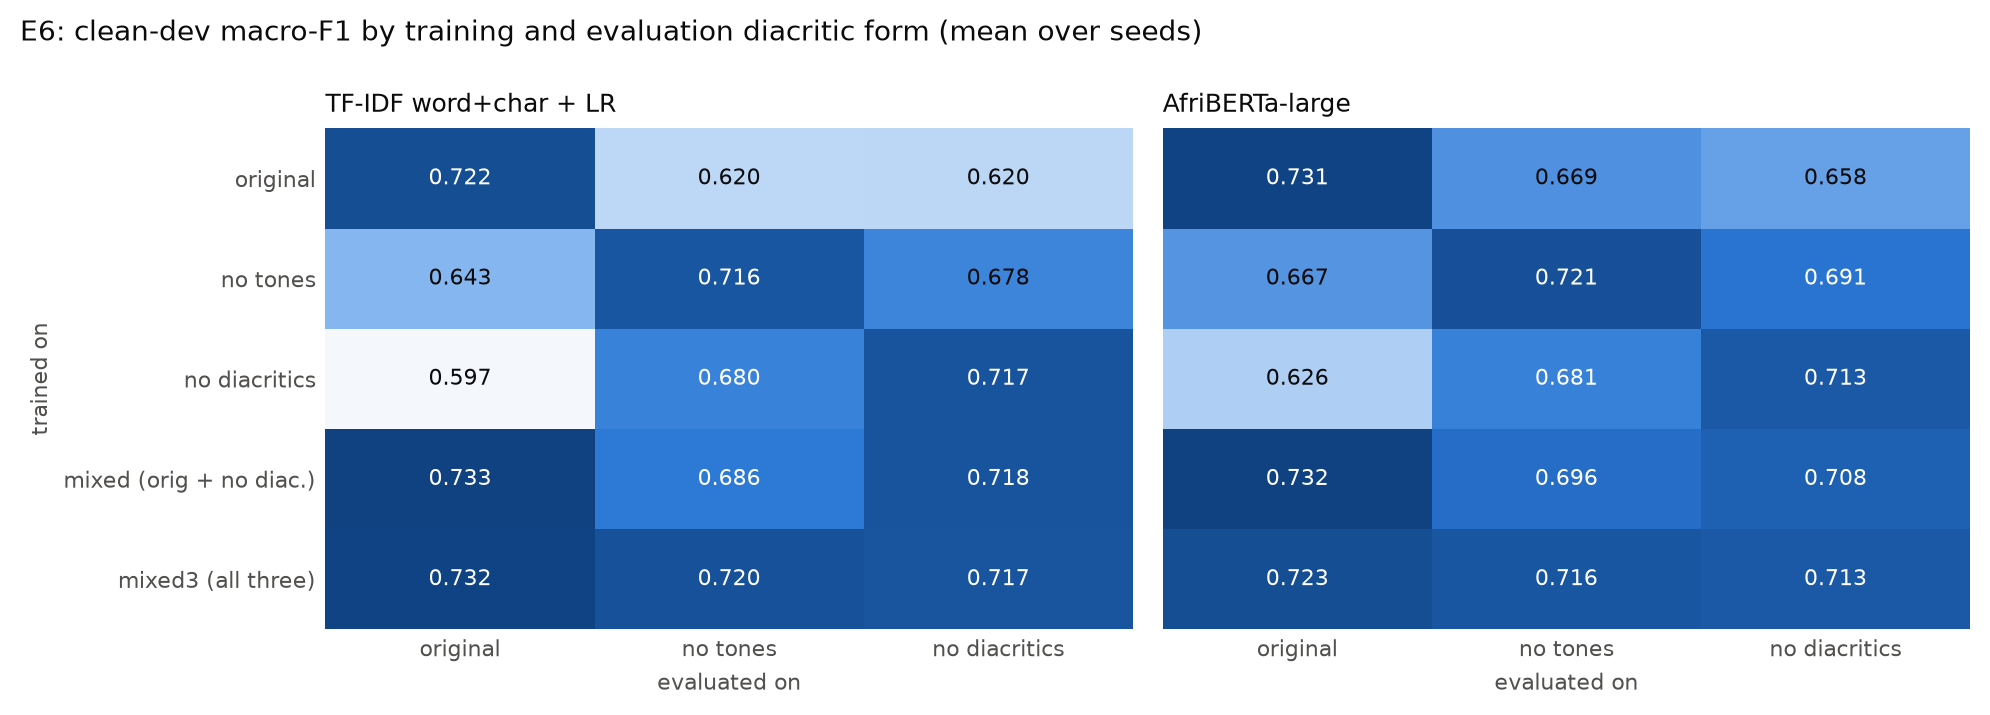
\includegraphics[width=0.9\textwidth]{e6_diacritic_matrix.png}
\caption{E6: clean-dev macro-F1 by training form (rows) and evaluation form (columns), mean over seeds.}
\label{fig:e6}
\end{figure*}

\paragraph{RQ2: diacritic robustness.} Models trained on original text are brittle (Figure~\ref{fig:e6}): removing tone marks at test time costs the baseline 10.3 points and AfriBERTa 6.2; removing all diacritics costs 10.2 and 7.3. Each model trained on a single form is best only on that form. Training on all three forms (\emph{mixed3}) gives near-uniform performance---0.732/0.720/0.717 for TF-IDF and 0.723/0.716/0.713 for AfriBERTa on original/no-tones/no-diacritics---with no meaningful loss on original text. AfroXLMR models are intrinsically robust to tone removal ($-0.6$ to $-1.4$) but still lose 4--6 points without under-dots.

\paragraph{RQ3 and other ablations.} Adding Hausa, Igbo and Pidgin data lowers Yorùbá performance to 0.716, and removing Pidgin (whose labels are skewed) does not help (0.715): diluting Yorùbá to about 30\% of the training mix, rather than the label prior, causes the negative transfer. Class weighting has no effect (0.729): the imbalance is mild and negative-class errors stem from ambiguity (§\ref{sec:errors}).

\begin{figure}[t]
\centering
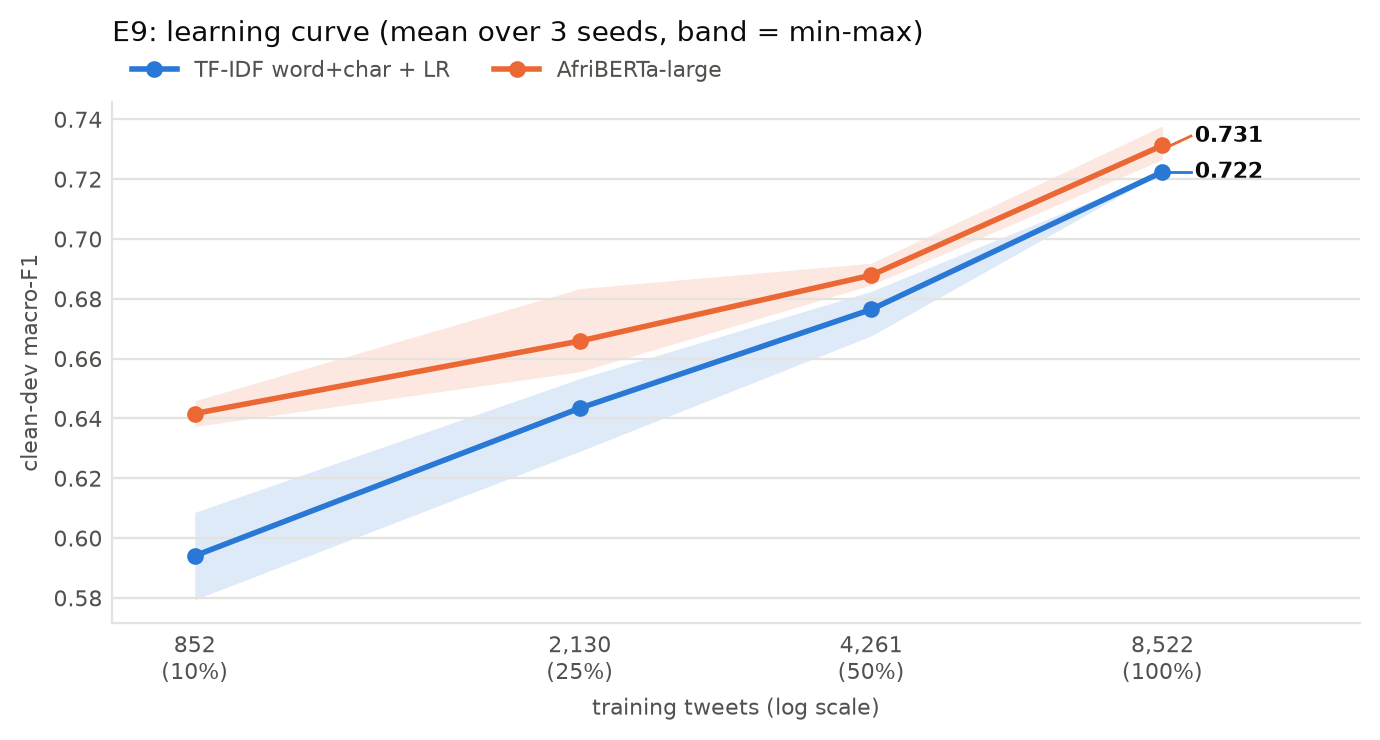
\includegraphics[width=\columnwidth]{e9_learning_curve.png}
\caption{E9: clean-dev macro-F1 vs.\ training-set size (3 seeds; band = min--max).}
\label{fig:e9}
\end{figure}

\paragraph{Learning curve.} Figure~\ref{fig:e9} explains why Transformers do not pull clearly ahead: AfriBERTa's advantage is largest with little labelled data (+4.8 points at 852 tweets) and shrinks to +0.9 at 8,522 tweets, as character n-grams catch up. Neither curve has plateaued.

\begin{table}[t]
\centering\small
\setlength{\tabcolsep}{2.8pt}
\begin{tabular}{lcccc}
\toprule
Model & mF1 (clean) & wF1 & $\Delta$tone & $\Delta$diac \\
\midrule
Majority & .197 & 25.3 & -- & -- \\
AfroXLMR-L + LoRA & .702\pmstd{.001} & 73.2 & $-$.001 & $-$.034 \\
BiLSTM+attn (E2g) & .710\pmstd{.005} & 74.7 & $-$.075 & $-$.085 \\
AfriBERTa-large & .732\pmstd{.005} & 76.7 & $-$.038 & $-$.070 \\
TF-IDF (E1c) & .737 & 77.2 & $-$.081 & $-$.084 \\
AfriBERTa, mixed3 & .741\pmstd{.007} & 77.5 & $-$.002 & $-$.012 \\
\textbf{TF-IDF, mixed3} & \textbf{.745} & \textbf{77.8} & +.001 & $-$.006 \\
\midrule
\multicolumn{5}{l}{\emph{Published, same test set (weighted-F1):}} \\
AfriBERTa-large$^{a}$ & -- & 72.9 & & \\
AfroXLMR-large$^{a}$ & -- & 74.1 & & \\
SemEval-2023 best$^{b}$ & -- & 80.2 & & \\
\bottomrule
\end{tabular}
\caption{Test results: clean-test macro-F1, all-test weighted-F1 ($\times$100, comparable to published numbers) and change in clean-test macro-F1 without tone marks / diacritics. $^{a}$\citet{muhammad-etal-2023-afrisenti}; $^{b}$\citet{muhammad-etal-2023-semeval}.}
\label{tab:test}
\end{table}

\paragraph{Test set.} Table~\ref{tab:test} confirms the dev findings: the model ranking is unchanged and dev-to-test differences are small ($-0.5$ to $+1.5$ points). The two \emph{mixed3} models are best and lose at most 1.2 points on undiacritised input, against 7--8 points without augmentation. No model significantly outperforms the TF-IDF baseline (paired bootstrap: best $p=0.055$ for TF-IDF mixed3; $p=0.13$--$0.87$ for the AfriBERTa mixed3 seeds). Our single models exceed the dataset's published single-model baselines by 3--5 weighted-F1 points, plausibly in part because we train on the same format as the test set; the SemEval winners used additional pre-training and ensembles.

\section{Error Analysis and Discussion}\label{sec:errors}
We analyse AfriBERTa (seed 42) against TF-IDF on clean test, using only reproducible evidence for quantitative claims.

\paragraph{Where errors occur.} Confusions are spread across all class pairs (most frequent: positive$\rightarrow$neutral, 219), and the negative class has the lowest F1. \textbf{64\% of AfriBERTa's errors (651 of 1,021) are shared with TF-IDF}, a hard core neither representation solves; each model fixes about 360 of the other's errors, so they are partly complementary. Table~\ref{tab:slices} reports objective slices: code-switched tweets and undiacritised tweets cost 5--6 points, and negation (\emph{kò}, \emph{kì í}) drops accuracy to 0.69 (TF-IDF 0.66) against 0.75 overall.

\begin{table}[t]
\centering\small
\setlength{\tabcolsep}{3pt}
\begin{tabular}{lrcc}
\toprule
Slice (clean test) & n & AfriBERTa & TF-IDF \\
\midrule
All & 4,129 & .753\,acc & .757\,acc \\
Code-switched (vs.\ not) & 556 & .690 / .744 & .696 / .743 \\
No diacritics (vs.\ with) & 813 & .693 / .741 & .681 / .741 \\
Negation \emph{kò / kì í} & 439 & .692\,acc & .663\,acc \\
Religious/greeting words & 463 & .911\,acc & .909\,acc \\
Negative-content words & 86 & .744\,acc & .744\,acc \\
\bottomrule
\end{tabular}
\caption{Error slices (macro-F1 unless marked acc = accuracy).}
\label{tab:slices}
\end{table}

\paragraph{Keyword priors.} 84\% of tweets containing religious or greeting words (\emph{Ọlọ́run, Olúwa, àdúrà, ẹ kú}) are positive, so models learn ``God $\Rightarrow$ positive'': half of their errors on such tweets (20/41) are false positives, e.g.\ a Bible verse (\emph{Ní àtètèkọ́ṣe Ọlọ́run dá ọ̀run àti ayé}, gold neutral). Symmetrically, 77\% of errors on tweets with words such as \emph{ikú} `death' or \emph{àrùn} `disease' follow the negative word, e.g.\ positive news about a rescue from Boko Haram.

\paragraph{Label noise.} Two reproducible signals indicate that part of the remaining error lies in the labels. First, 15 of the 386 test tweets that duplicate a training tweet carry a \emph{different} gold label, and AfriBERTa predicts the training copy's label in all 15 (one is a condolence message, labelled negative in train but positive in test). Second, confident learning \citep{northcutt-etal-2021-confident} with out-of-fold TF-IDF probabilities flags 10.8\% of training tweets (14.0\% of negatives) and 9.4\% of test tweets as likely label issues, consistent with the moderate inter-annotator agreement ($\kappa=0.65$). Flags are candidates, not proof, but they suggest roughly 10\% of the error is not reachable by any model trained on these labels.

\paragraph{Idioms, proverbs and calibration.} Reading the sampled errors (model-assisted glosses, not verified by a native speaker, so used only illustratively) shows sentiment carried by idioms and proverbs: \emph{àkàrà tú sépo} (`the bean cake has dissolved in the oil', i.e.\ things fell apart) is negative but predicted neutral; \emph{bójú bá farabalẹ̀ á rímú} (`if the eye is patient it will see the nose') is positive but predicted negative. Educational posts that quote a proverb are labelled by the proverb's content, the model often by the post's neutral style. AfriBERTa is also over-confident: 94\% of its test predictions have probability above 0.9, but only 77\% of those are correct \citep{guo-etal-2017-calibration}.

\paragraph{Discussion.} With 8.5k noisy, short tweets, a well-tuned character-aware n-gram model is a strong competitor to pre-trained Transformers; pre-training pays off most when labels are scarce, and African-language pre-training data matters more than model size, consistent with \citet{ogueji-etal-2021-small} and \citet{muhammad-etal-2023-afrisenti}. The practically most important result is cheap: rendering training data in all written forms makes both model families robust to how Yorùbá is actually typed.

\section{Deployment}
The deployed system (text input $\rightarrow$ training-identical normalisation $\rightarrow$ two classifiers $\rightarrow$ class probabilities) is a Streamlit application \citep{streamlit} on Streamlit Community Cloud. A user types or pastes a tweet, optionally simulates typing without tone marks or diacritics, and sees both mixed3 models' predicted labels and class probabilities side by side, the normalised text the models receive, and a warning when the models disagree. Example buttons include known hard cases. Input goes through exactly the training preprocessing code. The fine-tuned AfriBERTa (seed 42) and the TF-IDF model are published on the Hugging Face Hub with a model card. Because free Hugging Face hosting of Python applications now requires a paid plan and the free Streamlit tier offers about 1\,GB of memory, AfriBERTa is served as a per-channel int8 ONNX model with ONNX Runtime \citep{onnxruntime} (127\,MB, no PyTorch): on clean dev it agrees with the original model on 96.3--96.6\% of tweets and changes macro-F1 by at most 0.3 points; tokenisation is identical. The application uses about 550\,MB of memory and answers in about 0.05\,s per tweet.

\section{Limitations and Future Work}
\textbf{Data:} one domain (Twitter), three coarse classes, about 10\% suspected label noise and $\kappa=0.65$; no dialectal or Benin Yorùbá coverage. \textbf{Evaluation:} the test set is small for distinguishing models a few points apart; meaning-based error categories were not verified by a native speaker. \textbf{Models:} no Transformer significantly beats TF-IDF; probabilities are over-confident; negation and idioms remain unsolved. \textbf{System:} the free host sleeps after inactivity. \textbf{Future work:} native-speaker re-annotation of flagged tweets; language- and task-adaptive pre-training as used by the best SemEval systems \citep{wang-etal-2023-nlnde}; ensembling TF-IDF and AfriBERTa, whose errors are partly complementary; negation-aware augmentation; temperature-scaling calibration; and comparison with diacritic restoration \citep{orife-2018-attentive} as an alternative to augmentation.

\section{Conclusion}
We built and deployed a Yorùbá tweet sentiment classifier and found that the data, not the model, set most of the challenges: a hidden train/test format mismatch, duplicate leakage, label noise and diacritic variation. Africa-centric pre-training helps (RQ1), but on 8.5k tweets a well-tuned TF-IDF model is statistically indistinguishable from the best Transformer. Models trained on diacritised text are brittle to undiacritised input, and training on all written forms fixes this at no cost (RQ2). Data from related Nigerian languages did not help (RQ3). The main lessons are to audit the data before modelling, to evaluate with multiple seeds and significance tests, and to evaluate under the conditions in which a system will actually be used.

\section*{Use of Existing Resources and Own Contributions}
\textbf{Existing resources used:} the AfriSenti-SemEval~2023 data \citep{muhammad-etal-2023-afrisenti}; the pre-trained models mBERT, XLM-R, AfriBERTa and AfroXLMR; fastText Yorùbá vectors \citep{grave-etal-2018-learning}; Yorùbá Wikipedia text; and open-source libraries (PyTorch, Transformers, PEFT, scikit-learn, gensim, ONNX Runtime, Streamlit). \textbf{Implemented in this project:} the data pipeline (pinned loading, reconstruction and validation of the test normalisation, duplicate detection, diacritic transformations); all training, evaluation and analysis code (baselines, BiLSTM/BiGRU with attention, Word2Vec training and tiered embedding lookup, Transformer and LoRA fine-tuning, diacritic augmentation, bootstrap statistics, learning curves, error slices, confident-learning analysis); the reproducible Kaggle experiment pipeline; all 30+ experiments; and the deployment (model export and quantisation, validation, web application).

\bibliography{references}
\bibliographystyle{acl_natbib}

\end{document}
